\begin{problem}{2} ~\\
A node in the graph now has three possible assigned values instead of two. To represent the three possibilities, we can use three variables to represent the value of a node. In other words, a node A should has three variables in the formula: $A_1$, $A_2$ and $A_3$, representing value 1, 2 and 3 respectively.\\
\\
There are two conditions in order to reduce 3-colorability to Formula-sat: one is every node should only be assigned one of three values; the other is two vertexes of an edge should be assigned different values.\\
\\
For the following graph, to ensure node A only has one value assigned, it can be interpreted as $(A_1 \wedge \neg A_2 \wedge \neg A_3) \lor (\neg A_1 \wedge A_2 \wedge \neg A_3) \lor (\neg A_1 \wedge \neg A_2 \wedge A_3)$. To ensure vertexes of edge e1 are assigned different values, it can be interpreted as $(A_1 \wedge B_2) \lor (A_1 \wedge B_3) \lor (A_2 \wedge B_1) \lor (A_2 \wedge B_3) \lor (A_3 \wedge B_1) \lor (A_3 \wedge B_2)$.\\
\\
The whole graph can be interpreted as: $Clause 1 \wedge Clause 2 \wedge Clause 3 \wedge Clause 4 \wedge Clause 5$\\
\tab $Clause 1: (A_1 \wedge \neg A_2 \wedge \neg A_3) \lor (\neg A_1 \wedge A_2 \wedge \neg A_3) \lor (\neg A_1 \wedge \neg A_2 \wedge A_3)$\\
\tab $Clause 2: (B_1 \wedge \neg B_2 \wedge \neg B_3) \lor (\neg B_1 \wedge B_2 \wedge \neg B_3) \lor (\neg B_1 \wedge \neg B_2 \wedge B_3)$\\
\tab $Clause 3: (C_1 \wedge \neg C_2 \wedge \neg C_3) \lor (\neg C_1 \wedge C_2 \wedge \neg C_3) \lor (\neg C_1 \wedge \neg C_2 \wedge C_3)$\\
\tab $Clause 4: (A_1 \wedge B_2) \lor (A_1 \wedge B_3) \lor (A_2 \wedge B_1) \lor (A_2 \wedge B_3) \lor (A_3 \wedge B_1) \lor (A_3 \wedge B_2)$.\\
\tab $Clause 5: (A_1 \wedge C_2) \lor (A_1 \wedge C_3) \lor (A_2 \wedge C_1) \lor (A_2 \wedge C_3) \lor (A_3 \wedge C_1) \lor (A_3 \wedge C_2)$.
\begin{figure}[H] 
\centering 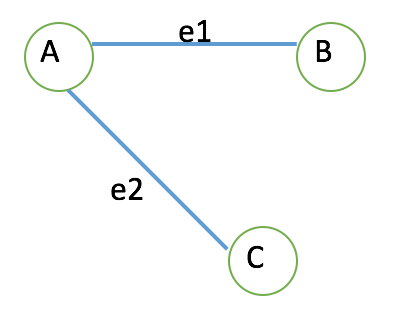
\includegraphics[width=0.4\columnwidth]{1_2}
\end{figure}
\end{problem}